%! Author = gramic
%! Date = 29.04.24

% Preamble
\begin{flushleft}
    \subsection{Architektur}
    Das Testsystem wird mit Patroni umgesetzt.\\
    Dabei werden folgende Komponenten eingesetzt:\\
    \begin{longtable}[H]{ll}

\toprule
Aufgabe & System \\
\midrule
\endfirsthead
\caption[]{Testsystem - Komponenten} \\
\toprule
Aufgabe & System \\
\midrule
\endhead
\midrule
\multicolumn{2}{r}{Continued on next page} \\
\midrule
\endfoot
\bottomrule
\endlastfoot
Orchestrator & Patroni \\
Proxy & Haproxy \\
\Gls{Connection Pooler} & PgBouncer \\
\Gls{DCS} & \gls{etcd} \\
\caption{Testsystem - Komponenten} \label{construction_components}
\end{longtable}

\end{flushleft}
\begin{flushleft}
    Entsprechend sieht das Architekturschema aus:
    \begin{figure}[H]
        \centering
        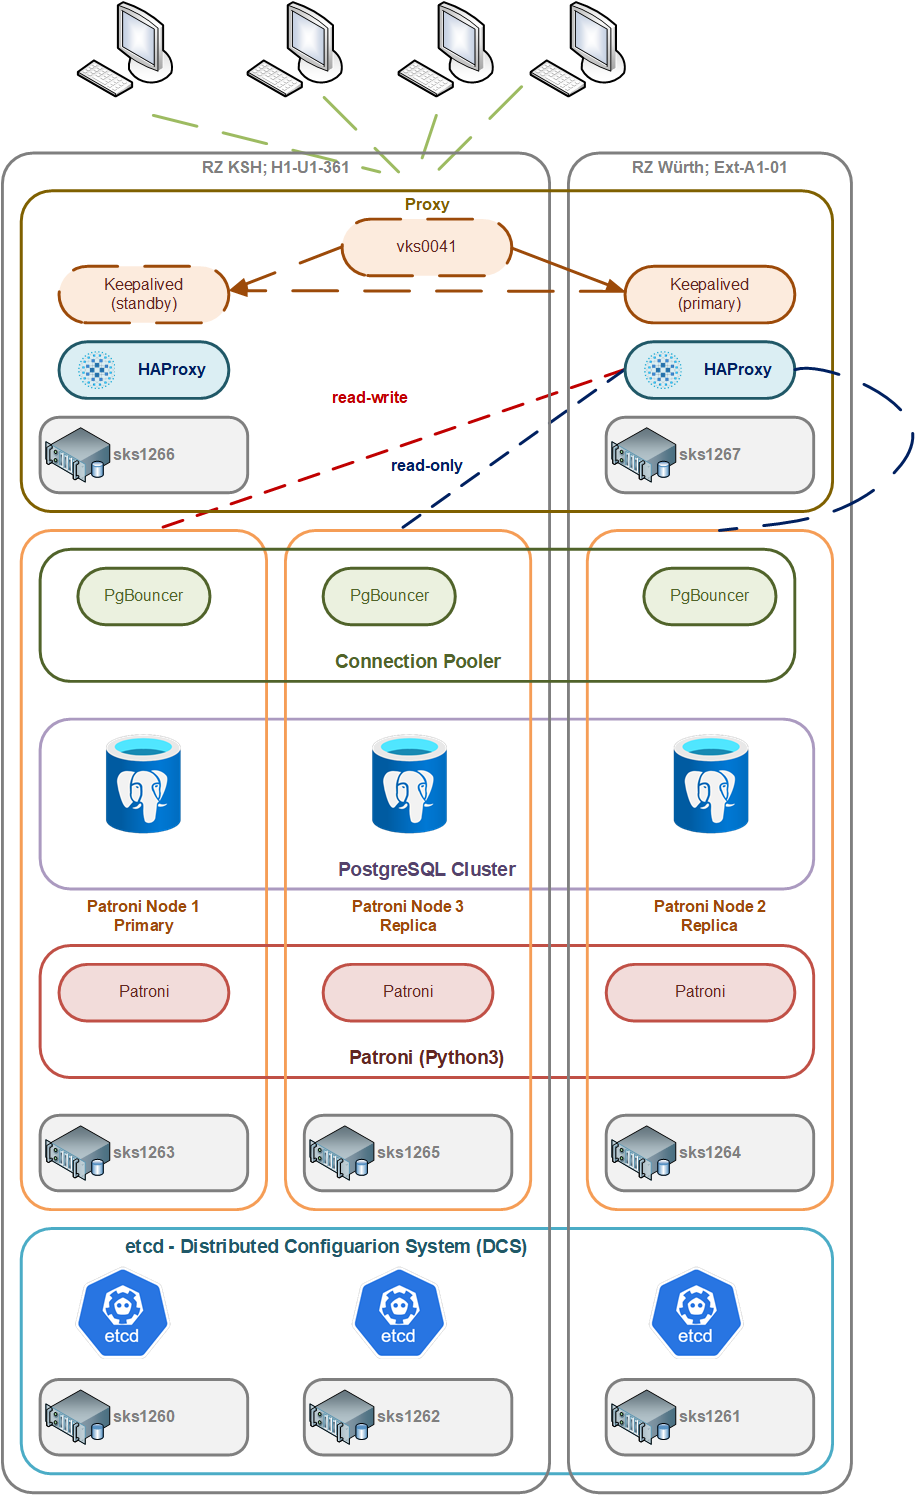
\includegraphics[width=0.75\linewidth]{source/implementation/construction_implementation/patroni-construction-architecture}
        \caption{Testsystem - Architektur}
        \label{fig:patroni-construction-architecture}
    \end{figure}
\end{flushleft}
\begin{flushleft}
    Folgende Server stehen daher im Einsatz:
    \begin{longtable}[H]{llllll}

\toprule
Server & Typ & Funktion & Full Qualified Device Name & Domain & IP \\
\midrule
\endfirsthead
\caption[]{Testsystem - Inventar} \\
\toprule
Server & Typ & Funktion & Full Qualified Device Name & Domain & IP \\
\midrule
\endhead
\midrule
\multicolumn{6}{r}{Continued on next page} \\
\midrule
\endfoot
\bottomrule
\endlastfoot
sks1260 & Monolith & etcd Node 1 & sks1260.ksgr.ch & ksgr.ch & 10.0.22.170 \\
sks1261 & Monolith & etcd Node 2 & sks1261.ksgr.ch & ksgr.ch & 10.0.22.171 \\
sks1262 & Monolith & etcd Node 3 & sks1262.ksgr.ch & ksgr.ch & 10.0.22.172 \\
sks1263 & Monolith & Database Node 1 & sks1263.ksgr.ch & ksgr.ch & 10.0.22.173 \\
sks1264 & Monolith & Database Node 2 & sks1264.ksgr.ch & ksgr.ch & 10.0.22.174 \\
sks1265 & Monolith & Database Node 3 & sks1265.ksgr.ch & ksgr.ch & 10.0.22.175 \\
sks1266 & Monolith & Pooler / Proxy Node 1 & sks1266.ksgr.ch & ksgr.ch & 10.0.22.176 \\
sks1267 & Monolith & Pooler / Proxy Node 2 & sks1267.ksgr.ch & ksgr.ch & 10.0.22.177 \\
vks0041 & Monolith & VirtualIP & vks0041.ksgr.ch & ksgr.ch & 10.0.22.178 \\
\caption{Testsystem - Inventar} \label{construction_inventory}
\end{longtable}

\end{flushleft}